\section{Operator}
\label{sec:komponenten:operator}

Operatoren oder auch Controller genannt, bieten die Möglichkeit, die Kubernetes API mit eigenen Typen und Funktionen zu erweitern .
Eigene Typen beziehungsweise \acp{CR} (\ref{subsection:kubernetes:customresource}) werden mittels einer \ac{CRD} erweitert.

\begin{figure}[h]
  \centering
  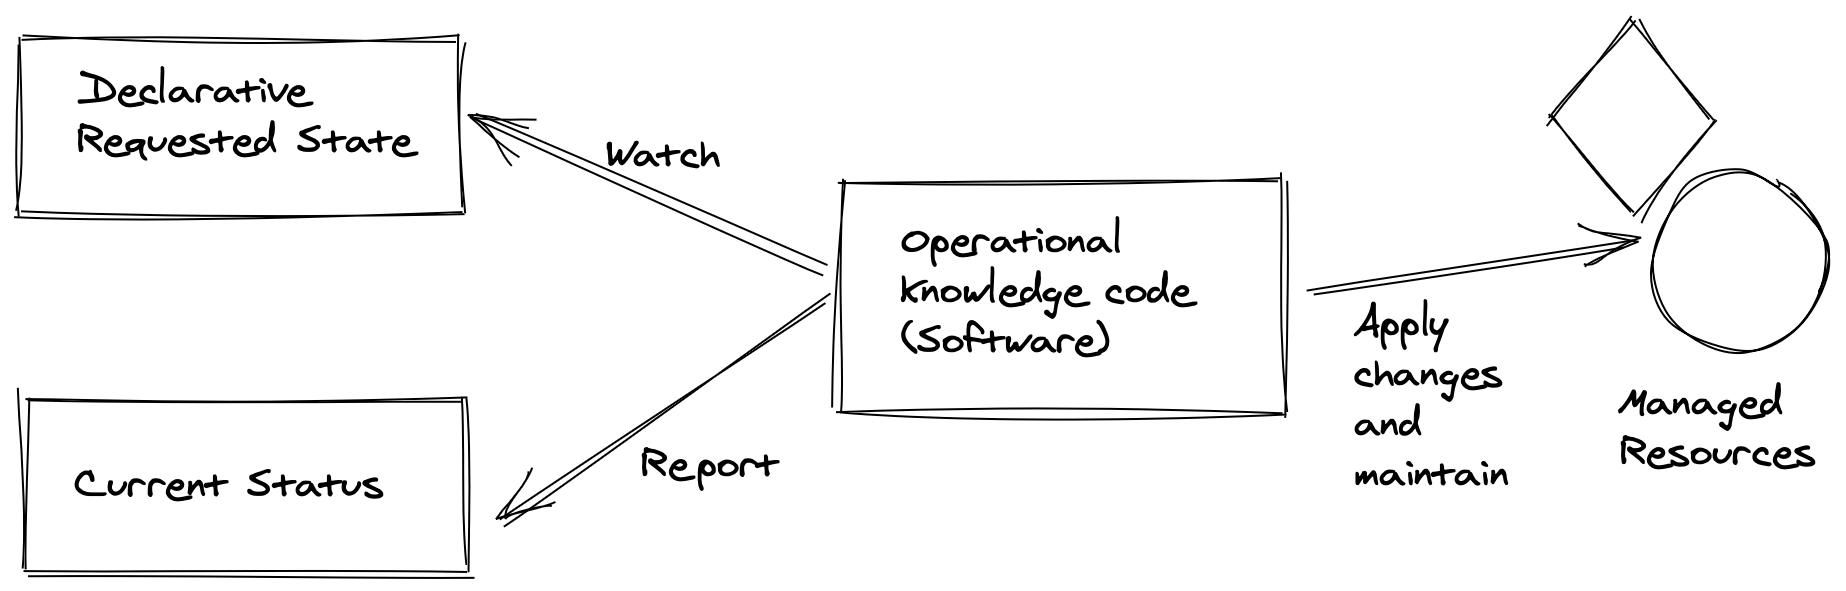
\includegraphics[width=\textwidth]{gfx/chapters/3_komponenten/operator_highlevel.png}
  \caption{High Level Überblick von Operatoren}
  \label{fig:kubernetes_operator_highlevel}
  \source{\cite{operatorWhitepaper}}
\end{figure}

Zur Verdeutlichung zeigt \ref{fig:kubernetes_operator_highlevel} einen abstrakten Überblick zu Operatoren.  
Durch Nutzen eines Controllers befindet sich jegliches Wissen zum Anpassen und Verwalten einer Ressourcen innerhalb des Anwendungcodes \cite{operatorWhitepaper}.

\begin{figure}[h]
  \centering
  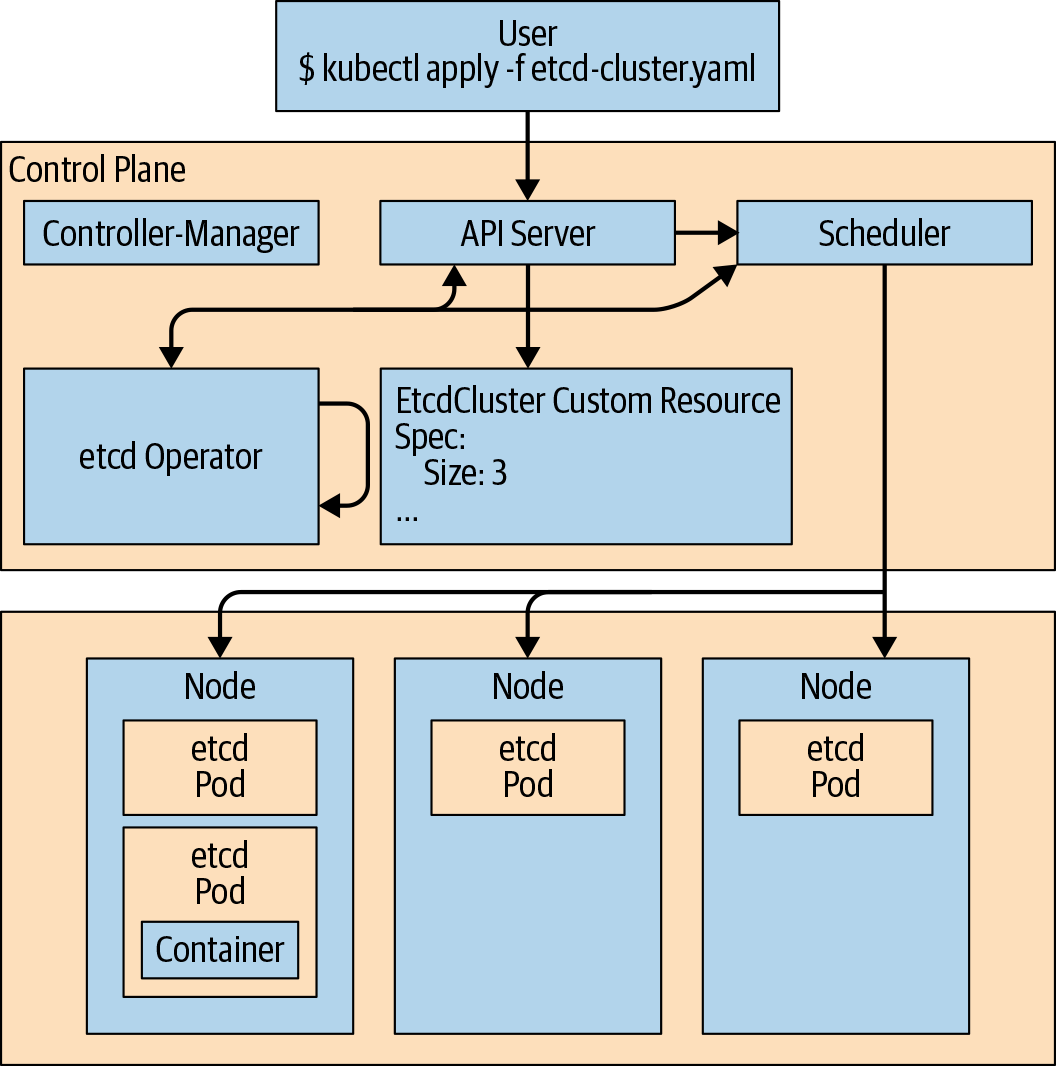
\includegraphics[width=\textwidth]{gfx/chapters/3_komponenten/operator_example.png}
  \caption{Funktionen eines Kubernetes Operators}
  \label{fig:kubernetes_operator_example}
  \source{\cite{Dobies2020}}
\end{figure}

In \ref{fig:kubernetes_operator_example} wird die Kommunikation des Operator im Cluster dargestellt.
Der Operator überwacht den API-Server auf Änderungen seiner zugewiesenen \ac{CR} Objekte. 
Auf Grundlage des Zustands der Objekte im Cluster ergreift er erforderliche Maßnahmen zur Erfüllung des gewünschten Zustands, 
wie beispielsweise das Erstellen neuer Pods \cite{Dobies2020}.
Diesen Synchronisationsmechanismus nennt man \emph{Reconciliation}.

Der für diese Referenzimplementation eines Chat \ac{SaaS} entwickelte Operator nutzt diesen Synchronisationsmechanismus,
um die Erstellung der RocketChat Anwendung zu vereinfachen. 
Der Rocket API Server erstellt ein \ac{CR} Objekt im Cluster und überlässt jegliche Verwaltung der eigentlichen Instanz dem Operator.
Operatoren können sich zusätzlich zur Bereitstellung und Konfiguration der Anwendung auch um die Funktionen Backup 
und automatische Reparatur des Services kümmern \cite{Dobies2020}.
Zur Einhaltung von validen Schemas des Objekts (\ref{subsection:kubernetes:customresource}),
wie beispielsweise die Nutzung eines existierenden Container Images für den Rocket Webserver,
kann ein \emph{Admission Controller} genutzt werden.
Die Funktion zur Erstellung von Backups sowie der Validierung durch einen Admission Controller
wurden allerdings in dieser Referenzimplementation nicht berücksichtigt wurden.


\paragraph{}
RocketChat Anwendungen bestehen aus einer MongoDB, welche als Replicaset konfiguriert wird,
sowie dem eigentlichen Webserver, welcher als Endpunkt für Clients dient.

Die Bereitstellung des Chat Services besteht aus den folgenden Kubernetes Objekten (\ref{sec:kubernetes:objekte}):
\begin{itemize}
  \item ConfigMap für MongoDB Scripts
  \item Secret für MongoDB Authentifizierung (Username und Passwort)
  \item Persistent Volume für MongoDB
  \item Service für Rocket.Chat und MongoDB Pods
  \item Deployment für Rocket.Chat Pods
  \item StatefulSet für MongoDB Pods
  \item Ingress für Rocket.Chat
  \item ServiceAccount
\end{itemize} 

\subsection{Rocket Custom Resource}
Als API für den Operator dient die Rocket \ac{CRD}. Diese wird im Code als Go Struct definiert, welches letztendlich
als JSON\footnote{\href{https://www.json.org/json-de.html}{JSON}} Objekt an die Kubernetes API gesendet wird.
Genauer dargestellt wird die Ressource in \ref{chap:rocketchat_crd_spec}, in dem aufgezeigt wird, wie das Objekt aufgebaut ist.
Nutzer des Kubernetes Cluster können selbst solche Rocket \acp{CR} via YAML oder JSON Dateien erstellen und
an die Kubernetes API schicken. Für diese \ac{SaaS} Anwendung ist dieser Anwendungsfall allerdings nicht vorgesehen.
Endnutzer sollen sich nicht mit der Komplexität von Kubernetes auseinander setzen müssen, 
sondern nur per Konfiguratorclient (\ac{CLI} oder Webinterface) ihren Chat Service erstellen.


